%%%%%%%%%%%%%%%%%%%%%%%%%%%%%%%%%%%%%%%%%
% Beamer Presentation
% LaTeX Template
% Version 1.0 (10/11/12)
%
% This template has been downloaded from:
% http://www.LaTeXTemplates.com
%
% License:
% CC BY-NC-SA 3.0 (http://creativecommons.org/licenses/by-nc-sa/3.0/)
%
%%%%%%%%%%%%%%%%%%%%%%%%%%%%%%%%%%%%%%%%%

%----------------------------------------------------------------------------------------
%	PACKAGES AND THEMES
%----------------------------------------------------------------------------------------

\documentclass[12pt]{beamer}
\mode<presentation> {

% The Beamer class comes with a number of default slide themes
% which change the colors and layouts of slides. Below this is a list
% of all the themes, uncomment each in turn to see what they look like.

%\usetheme{default}
%\usetheme{AnnArbor}
%\usetheme{Antibes}
%\usetheme{Bergen}
%\usetheme{Berkeley}
%\usetheme{Berlin}
%\usetheme{Boadilla}
%\usetheme{CambridgeUS}
%\usetheme{Copenhagen}
%\usetheme{Darmstadt}
%\usetheme{Dresden}
%\usetheme{Frankfurt}
%\usetheme{Goettingen}
%\usetheme{Hannover}
%\usetheme{Ilmenau}
%\usetheme{JuanLesPins}
%\usetheme{Luebeck}
\usetheme{Madrid}
%\usetheme{Malmoe}
%\usetheme{Marburg}
%\usetheme{Montpellier}
%\usetheme{PaloAlto}
%\usetheme{Pittsburgh}
%\usetheme{Rochester}
%\usetheme{Singapore}
%\usetheme{Szeged}
%\usetheme{Warsaw}

% As well as themes, the Beamer class has a number of color themes
% for any slide theme. Uncomment each of these in turn to see how it
% changes the colors of your current slide theme.

%\usecolortheme{albatross}
%\usecolortheme{beaver}
%\usecolortheme{beetle}
%\usecolortheme{crane}
%\usecolortheme{dolphin}
%\usecolortheme{dove}
%\usecolortheme{fly}
%\usecolortheme{lily}
%\usecolortheme{orchid}
%\usecolortheme{rose}
%\usecolortheme{seagull}
%\usecolortheme{seahorse}
%\usecolortheme{whale}
%\usecolortheme{wolverine}

%\setbeamertemplate{footline} % To remove the footer line in all slides uncomment this line
%\setbeamertemplate{footline}[page number] % To replace the footer line in all slides with a simple slide count uncomment this line

%\setbeamertemplate{navigation symbols}{} % To remove the navigation symbols from the bottom of all slides uncomment this line
}
\usepackage[utf8]{inputenc}
\usepackage{adjustbox}
\usepackage[T2A]{fontenc}
\usepackage{amssymb}
\usepackage{amsmath}
\usepackage{mathrsfs}
\usepackage{euscript}
\usepackage{upgreek}
\usepackage[english,russian]{babel}
\usepackage{array}
\usepackage{theorem}
\usepackage[all]{xy}
\usepackage{graphicx}
\usepackage{subfig}
\usepackage{epstopdf}   
\usepackage{tikz}       
\usepackage{pgfplots}   
\usepackage{color}
\usepackage{ifthen}
\usepackage{url}
\usepackage{makeidx}
\usepackage{pb-diagram}
\usepackage{balance}
\usepackage{multirow} 
\usepackage{bibentry}
\usepackage{graphicx} % Allows including images
\usepackage{booktabs}
\usepackage{graphics}
\usepackage{cmap}
\usepackage{amsthm}
\usepackage[linesnumbered,ruled,vlined]{algorithm2e}
\usepackage[absolute]{textpos}
\usepackage{fleqn,psfrag,wrapfig,tikz}
\usepackage{algpseudocode}
\usepackage{tabularx}
 
%----------------------------------------------------------------------------------------
%	TITLE PAGE
%----------------------------------------------------------------------------------------

\title[Достаточный объем выборки]{Раннее прогнозирование достаточного объема выборки для обобщенной линейной модели.} % The short title appears at the bottom of every slide, the full title is only on the title page

\author{Валентин Бучнев} % Your name
\institute[МФТИ] % Your institution as it will appear on the bottom of every slide, may be shorthand to save space
{
МФТИ\\ 
ФИВТ \\ % Your institution for the title page
\medskip
\textit{buchnev.valentin@gmail.com} % Your email address
}
\date{\today} % Date, can be changed to a custom date

\begin{document}

\begin{frame}
\titlepage % Print the title page as the first slide
\end{frame}

%----------------------------------------------------------------------------------------
%	PRESENTATION SLIDES
%----------------------------------------------------------------------------------------

\begin{frame}
\frametitle{Цели исследования}
\begin{block}{Цель работы}
Предложить метод предсказания достаточного объема выборки для обобщенной линейной модели.
\end{block}
\begin{block}{Проблема}
Большинство неассимптотических методов требуют заведомо большого объема выборки.
\end{block}
\begin{block}{Метод решения}
Модификация таких методов путем введения нескольких аппроксимаций для получения возможности  прогнозирования изменений зависимостей при увеличении размера выборки.
\end{block}

\end{frame}

\begin{frame}
\frametitle{Существующие методы}

\textbf{Ассимптотические методы}

\begin{itemize}
  \item S.\,G.\;Self and R.\,H.,\; Mauritsen Power/sample size calculations for generalized linear
models~//~Biometrics, 1988
  \item G.\,Shieh,\;On power and sample size calculations for likelihood ratio tests in generalized linear models~//~Biometrics, 2000.
  \item G.\,Shieh\;On power and sample size calculations for Wald tests in generalized linear models~//~Journal of Statistical Planning and Inference, 2005.
\end{itemize}

\textbf{Байесовские методы}

\begin{itemize}
  \item D.\,B.\;Rubin and H.\,S.\;Stern\;Sample size determination using posterior predictive distributions~//~Sankhya : The Indian Journal of Statistics Special Issue on Bayesian Analysis, 1998.
\end{itemize}

\end{frame}

\begin{frame}
\frametitle{Постановка задачи раннего прогнозирования}
\begin{block}{Дано}
Выборка размера m: $~\mathfrak D_m = \{\textbf{x}_i, y_i\}_{i=1}^m,$

где $\textbf{x}_i \in \mathbb{R}^{n}$ - вектор признаков, $~y_i \in \mathbb{Y}$.
\end{block}
\begin{block}{Функция правдоподобия}
Определим функцию правдоподобия и логарифмическую функцию правдоподобия выборки $\mathfrak D$:
$$
L(\mathfrak{D}, \textbf{w}) = \prod_{y, \textbf{x} \in \mathfrak D} f(y, \textbf{x}, \textbf{w}),~~~ l(\mathfrak D, \textbf w) = \sum_{y, \textbf{x} \in \mathfrak D}\log f(y, \textbf{x}, \textbf{w}),
$$
где $f(y, \textbf{x}, \textbf{w})$ - аппроксимация плотности апостериорной вероятности выборки $\mathfrak D_{\mathcal L_m}$ при заданном векторе параметров $\textbf{w}$.
\end{block}
\end{frame}

\begin{frame}
\frametitle{Постановка задачи раннего прогнозирования}
\begin{block}{Логарифмическая функция правдоподобия}
Будем рассматривать ожидаемое значение функции $l$:

$$
\tilde{l}(\mathfrak D)  = \underset{y, \textbf{x} \in \mathfrak D}{\mathsf E} l(\{y, \textbf{x}\}, \textbf w).
$$
\end{block}
\begin{block}{Ожидаемое значение}
Рассмотрим ожидаемое значение логарифма правдоподобия по разным обучающим выборкам $\mathfrak D_{\mathcal L_m}$ размера $m^*$:

$$
l(m^*) = \underset{\mathfrak D_{\mathcal L_m}}{\mathsf E} \tilde{l}(\mathfrak D_{\mathcal L_m}).
$$
\end{block}
\end{frame}


\begin{frame}
\frametitle{Постановка задачи раннего прогнозирования}
\begin{block}{Критерий достаточности объема}
Будем считать, что объем выборки достаточный, если:

$$
\forall m_1, m_2 > m^* ~~~ |l(m_1) - l(m_2)| < \varepsilon,
$$
где $\varepsilon$ - достаточно малое пороговое значение.
\end{block}
\end{frame}

\begin{frame}
\frametitle{Предлагаемый метод решения}

\begin{block}{Критерий средней длины}
$$
A(\mathfrak{D}) = \{\textbf{w} : ||\textbf{w}- \hat{\textbf{w}}|| \leqslant r_m\}
$$
$$
\mathsf{P}(A(\mathfrak{D})) = 1 - \alpha,
$$
где $\alpha$ --- некоторое малое значение. 

Критерий средней длины выглядит следующим образом:

$$
\forall m \geqslant m^{*}~\mathsf{E}_{\mathfrak D_m} r_m \leqslant l , 
$$
где $r_m$ --- радиус шара $A(\mathfrak{D}_m)$, $l$ --- некоторое наперед заданное достаточно малое значение.
\end{block}
\end{frame}

\begin{frame}
\frametitle{Предлагаемый метод решения}
\begin{block}{Модификация критерия}
Предлагается заменить ковариационную матрицу вектора параметров на её аппроксимацию через матрицу информации Фишера, далее строить аппроксимацию зависимости значения функции эффективности от размера выборки.
\end{block}
\end{frame}

\begin{frame}
\frametitle{Вычислительный эксперимент}
\begin{block}{Цель эксперимента}
Проверить работоспособность предложенного метода.
\end{block}

$\newline$

\textbf{Выборки из UCI репозитория.}

\begin{table}[h!]
\begin{center}
\label{table2}
\begin{tabularx}{\textwidth}{|p{1in}|X|X|c|}
\hline
	\centering Выборка &\centeringТип задачи&\centering Размер выборки& Число признаков\\
	\hline
	Servo &регрессия&\centering167&4\\
	\hline
	Boston &регрессия&\centering506&13\\
	\hline
	Diabetes&регрессия&\centering 442&5\\
\hline
\end{tabularx}
\end{center}
\end{table}
\end{frame}

\begin{frame}
\frametitle{Результаты}
\begin{figure}[h!t]\center
\subfloat[Servo]{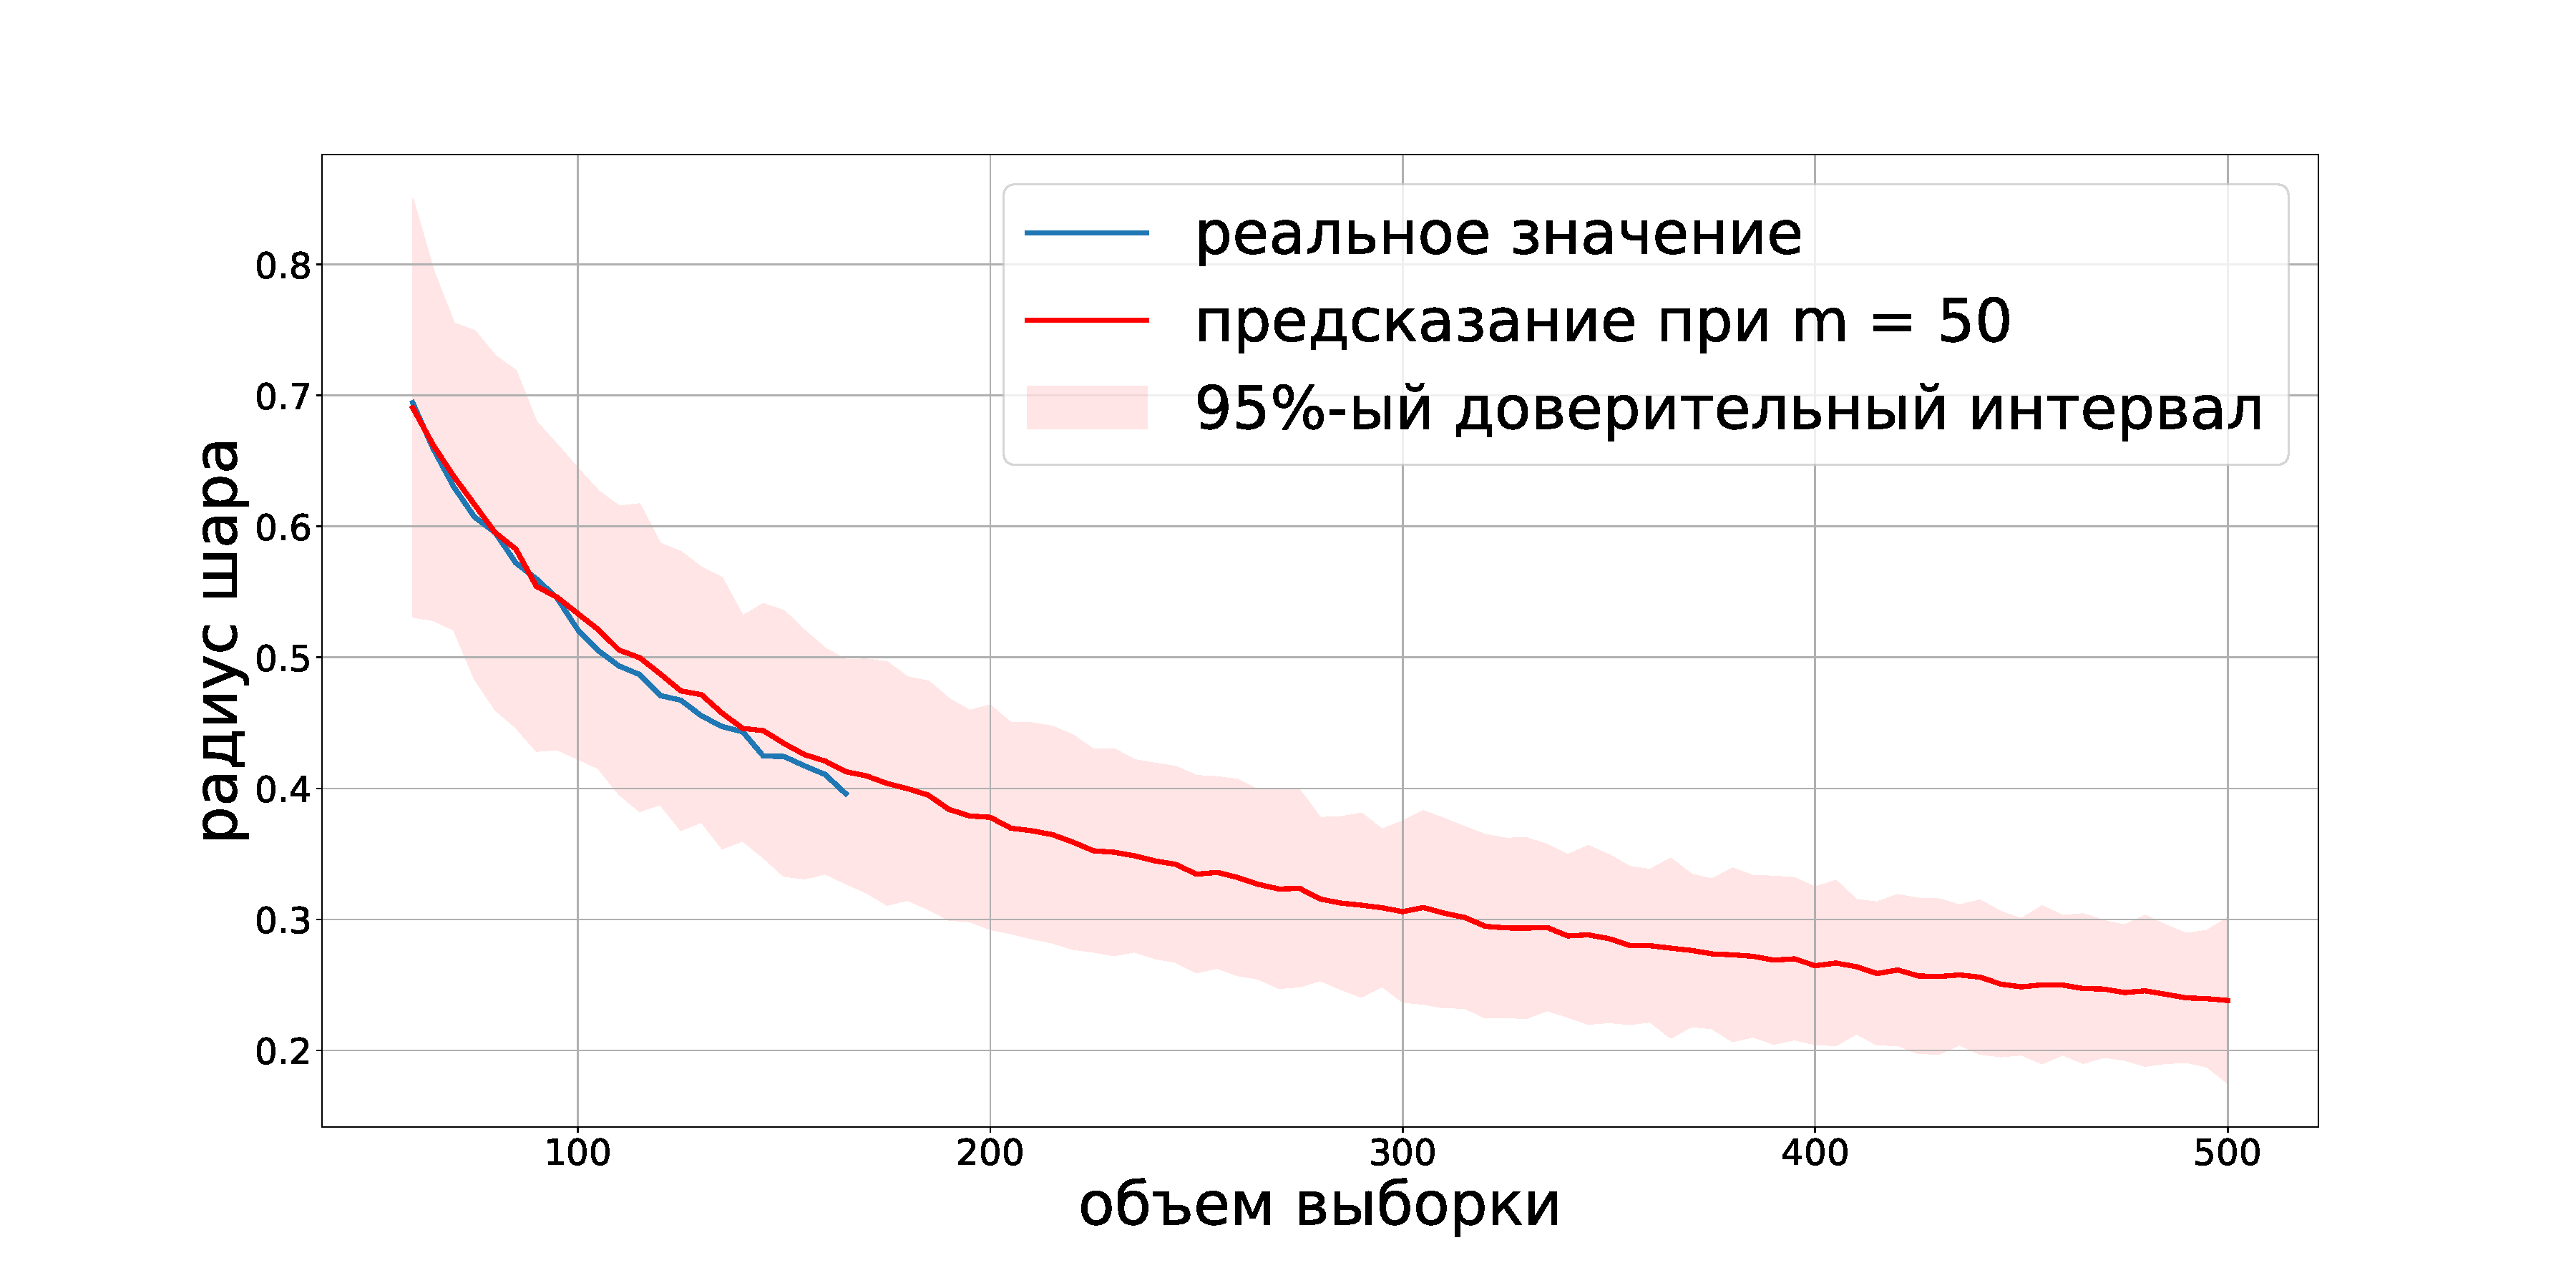
\includegraphics[width=0.5\textwidth]{../data/pics/ALC_modified_servo.pdf}}
\subfloat[Boston]{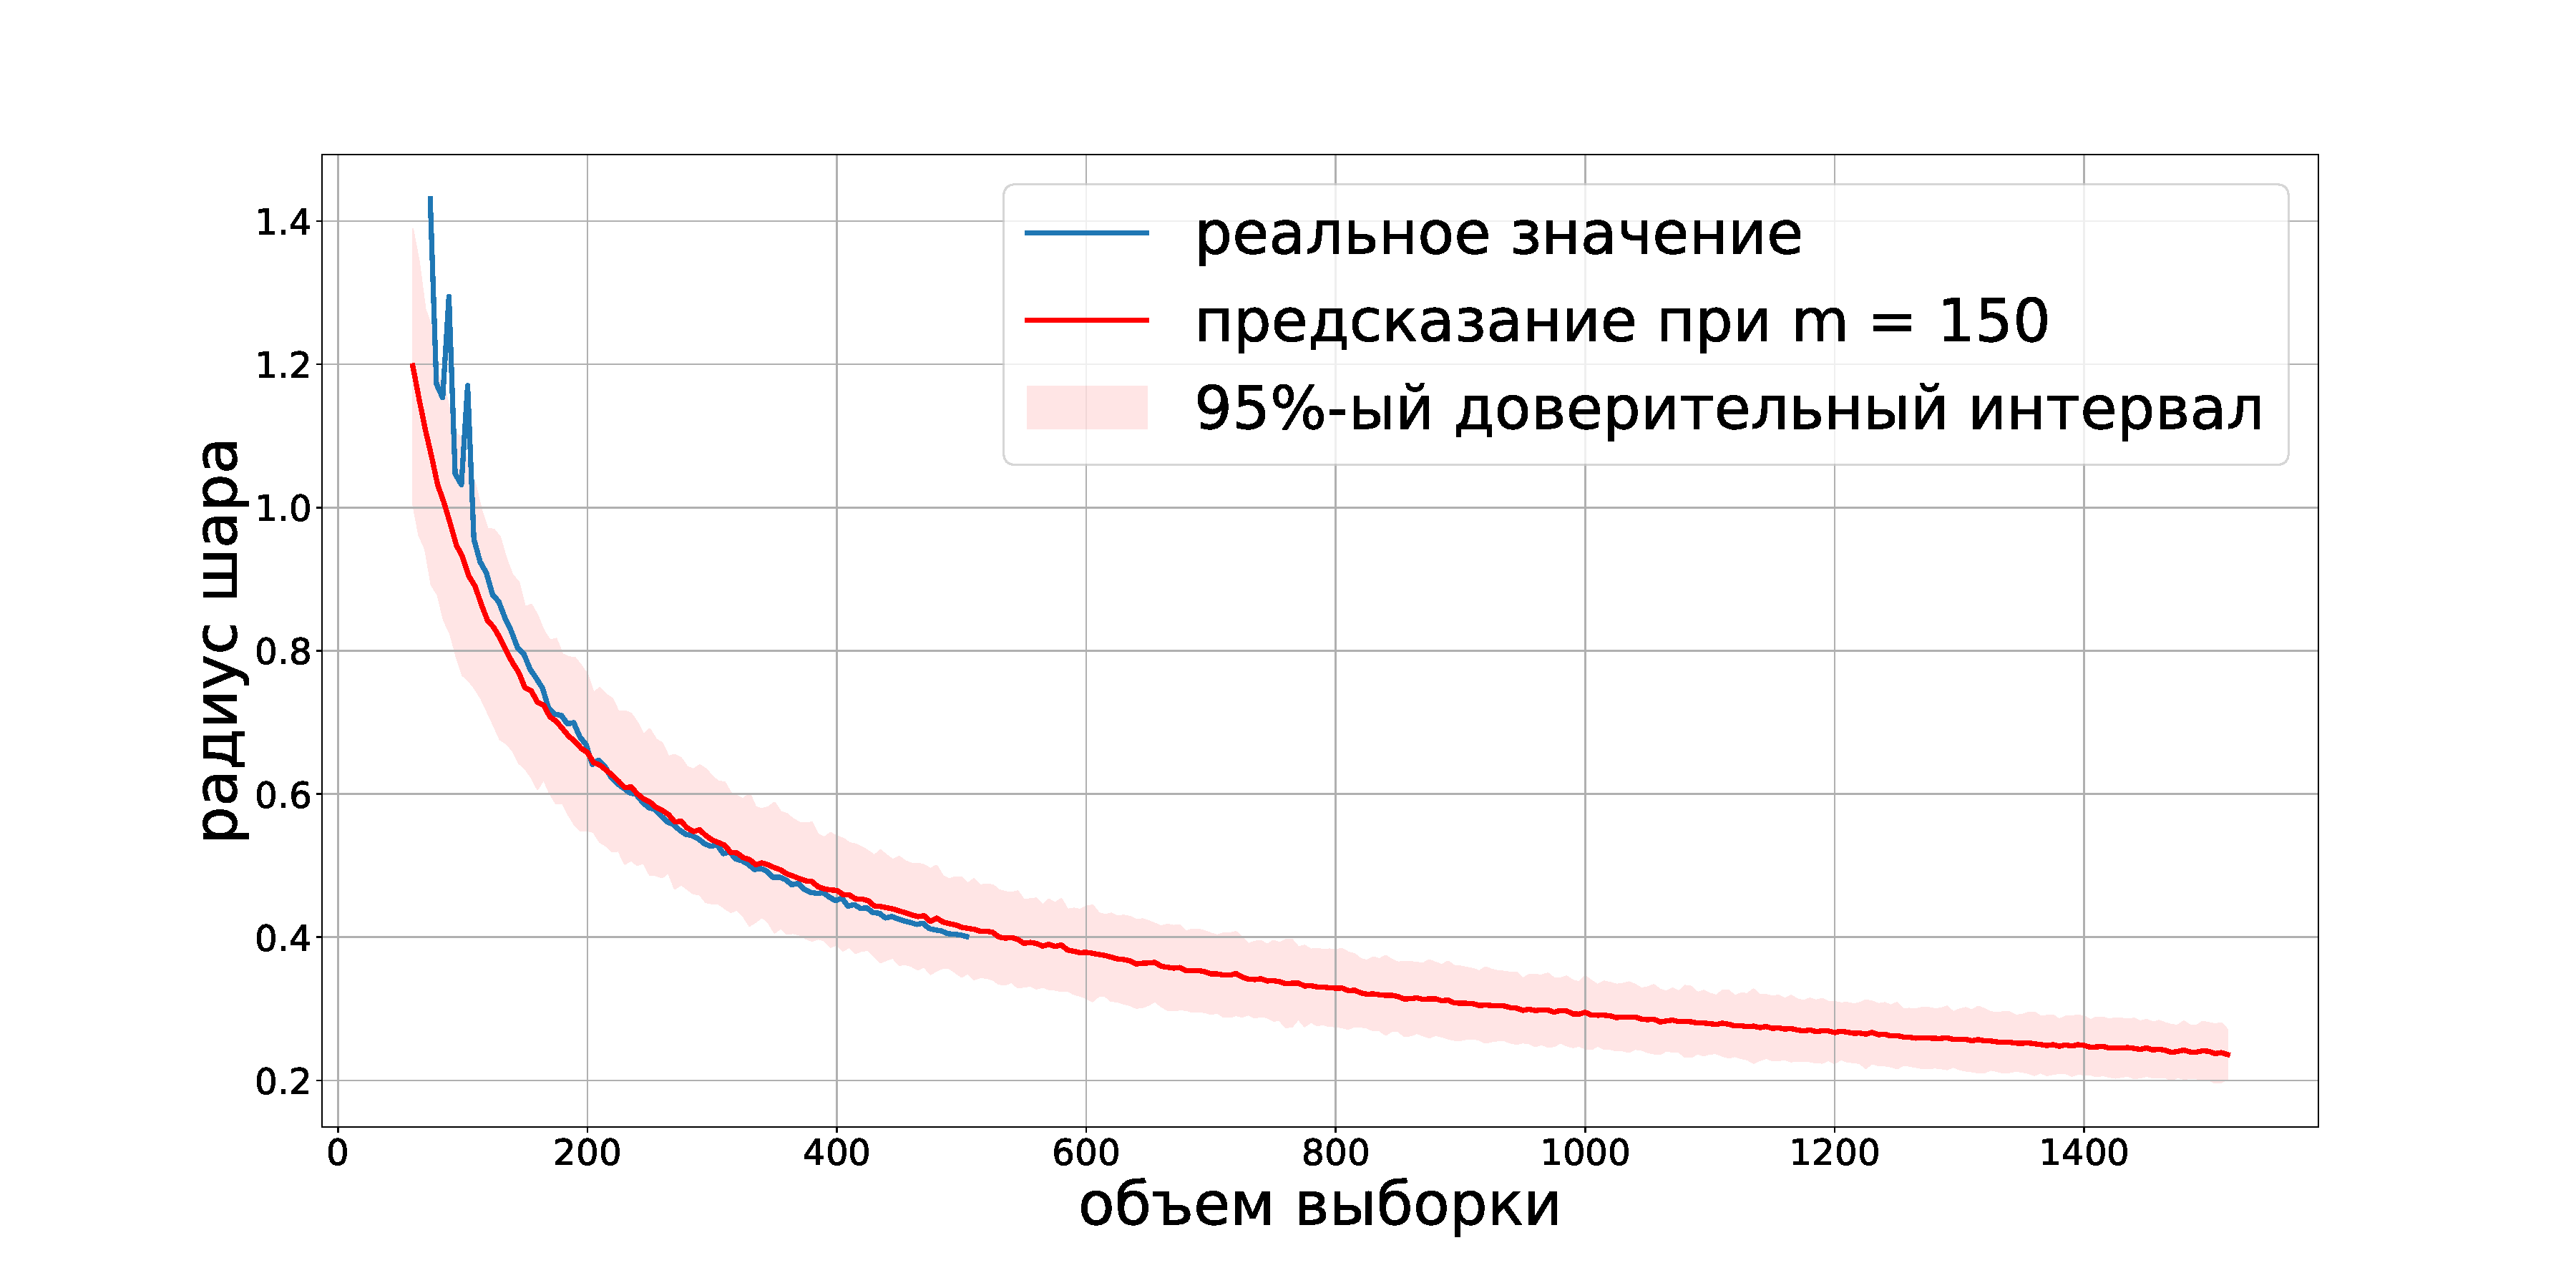
\includegraphics[width=0.5\textwidth]{../data/pics/ALC_modified_boston.pdf}}\\
\subfloat[Diabetes]{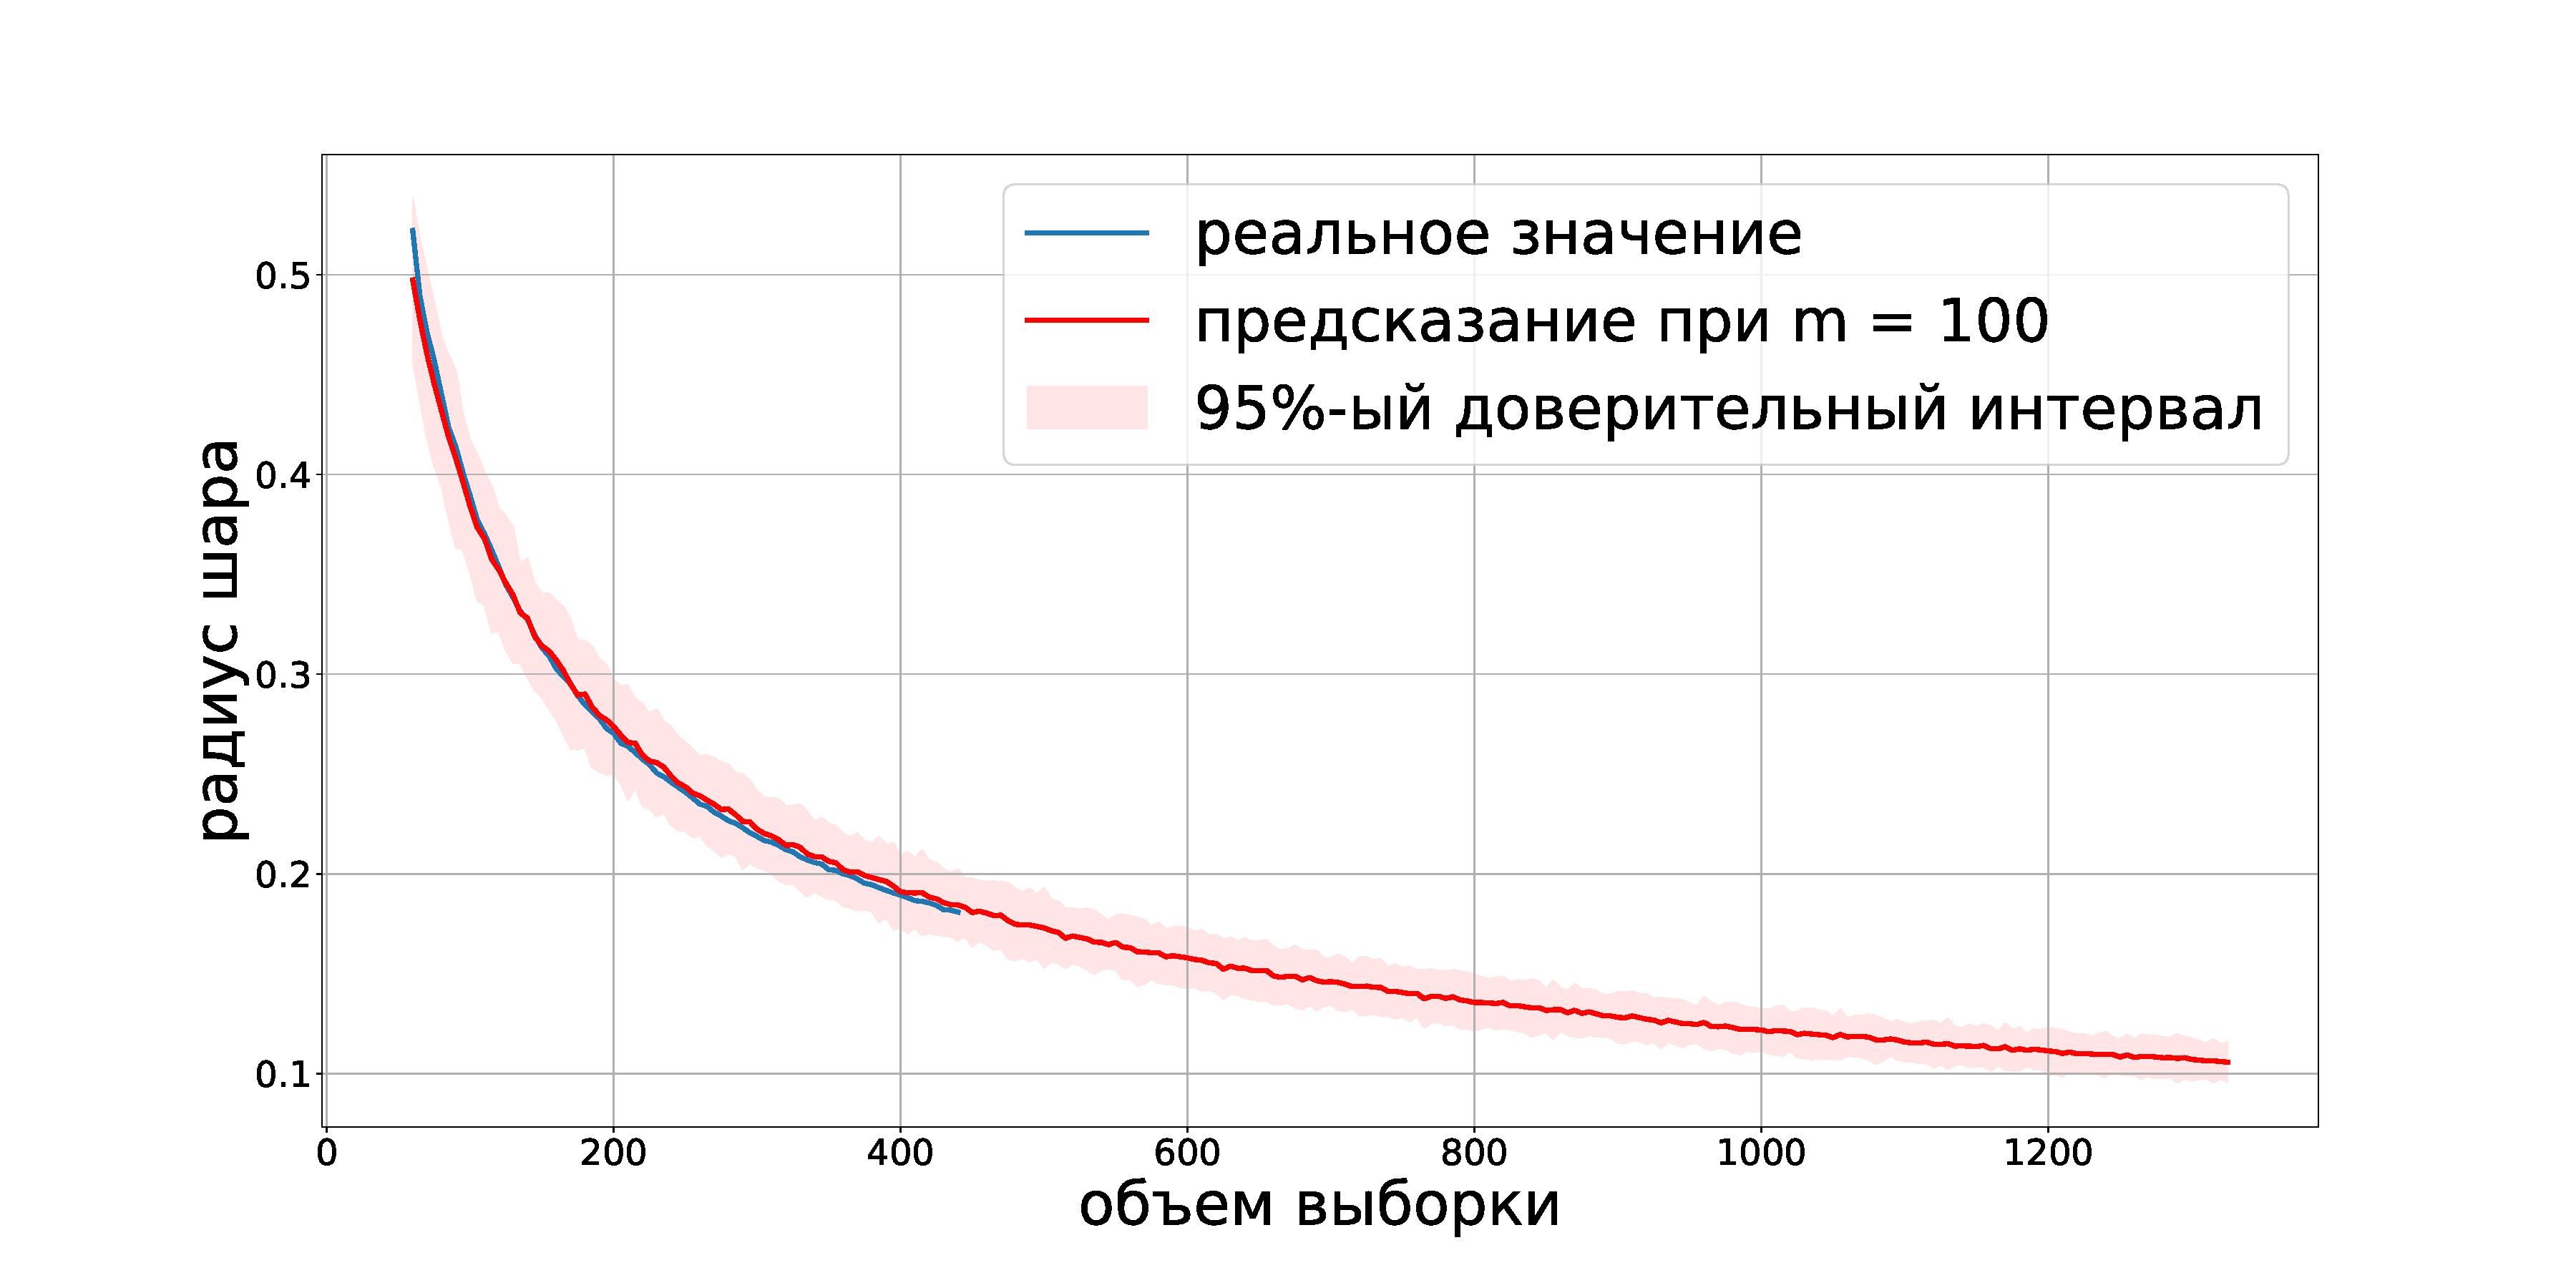
\includegraphics[width=0.5\textwidth]{../data/pics/ALC_modified_diabetes.pdf}}\\

\caption{ALC метод}
\label{fig1}
\end{figure}
\end{frame}

\begin{frame}
\frametitle{Заключение}

\begin{itemize}
  \item Задача прогнозирования достаточного объема выборки сведена к задаче аппроксимации корреляционной матрицы вектора параметров.
  \item Показана работоспособность предложенного метода на тестовых выборках.
  \item Далее можно строить аппроксимацию зависимости ожидаемого значения логарифма правдоподобия от размера выборки.
\end{itemize}

\end{frame}

\end{document}